\documentclass{article}
\usepackage{graphicx}
\usepackage{amsmath}
\usepackage{hyperref}

\DeclareFontFamily{OT1}{cmtt}{\hyphenchar \font=-1}
\DeclareFontFamily{\encodingdefault}{\ttdefault}{\hyphenchar\font=`\-}

\author{Martijn Dwars (4156730) \and Rik Nijessen (4152263)}

\title{Assignment 2 \\ Software Reengineering (IN4189)}

\begin{document}

\maketitle

\section{Introduction}
In our previous report we have analysed the architecture and the shortcomings of the implementation of the Alitheia Core software project. In this report we will describe which shortcomings we have addressed and how this influences the maintainability of the project.
We have used the Intellij plugin Metrics Reloaded \footnote{\url{https://plugins.jetbrains.com/plugin/93?pr=idea}} to assess the quality of our improvements. We have focussed on the following metrics:
\begin{description}
\item[Average operation complexity] The average cyclomatic complexity of a class.
\item[Weighted method complexity] The total cyclomatic complexity of a class.
\item[Number of cyclic dependencies]  The number of classes or interfaces which each class directly or indirectly depends on and which in turn directly or indirectly depend on it. 
\item[Number of dependencies] The number of classes or interfaces which each class directly depends on.
\item[Number of dependents] The number of classes or interfaces which directly depend on each class.
\end{description}

\subsection{SRP: Bug knows too much}
In our previous report we have found that the \verb|Bug| class has multiple responsibilities. This class' main job is to represent the concept of a bug. However, in its current state it also aware of the way it is persisted in the database.
This is a violation of SRP, because the \verb|Bug| class represents a bug but also contains functionality for retrieving bugs from the database. This is a shortcoming, because classes with many responsibilities are harder to maintain~\cite{martin2003agile}.

We implemented the Repository Pattern~\cite{repository} by creating the class \verb|BugRepository|. This class sits between the domain (i.e. \verb|Bug|) and data mapping layer (i.e. Hibernate) containing SQL queries.
This results in two seperate classes which each have there own responsibilities. This makes the code easier to maintain, because there is only one reason to change a class and therefore functionality~\cite{martin2003agile}.
The metrics mentioned in the introduction are not relevant for this refactoring. We where not able to find relevant metrics for this kind of change.


\subsection{SRP: Job knows how to execute itself}
The second Single Responsibility Principle violation we solved is the \verb|Job| class. This class represents the concept of a job, but also contains the implementation to run itself. This gives the \verb|Job| class multiple reasons to change and is therefore hard to maintain.
We split this into \verb|Job| representing the concept of a job and \verb|JobExecutor| which contains the implementation to execute a job. The metrics mentioned in the introduction are not relevant for this refactoring. We where not able to find relevant metrics for this kind of change.


\subsection{DIP: depend on abstractions (1)}
First we renamed \verb|InMemoryDirectory| to \verb|InMemoryDirectoryImpl|. We then created an \texttt{InMemoryDirectory} interface and made \verb|InMemoryDirectoryImpl| implement it. Finally, we replaced all expectations of type \verb|InMemoryDirectoryImpl| by expectations of type \verb|InMemoryDirectory|.

What is the violation and which classes/packages are involved in the violation? Why is it a shortcoming?
 -> DIP. DIP is a form of decoupling software modules. More decoupled software is better maintainable. For example, if you want to add a new cache service, you need to modify the \verb|CacheServiceImpl| as well as your new implementation.

We renamed \verb|CacheServiceImpl| to \verb|BaseCacheServiceImpl| and removed code that was responsible for the dependency inversion. As part of our solution we use the \verb|Activator| to register an implementation of the \verb|CacheService| (depending on the system property \verb|CACHE_IMPL|).

Another shortcoming in the old code was that the constant \verb|CACHE_IMPL| was used as key for a system property describing the actual implementation. However, it had the value \texttt{eu\allowbreak.sqooss.service.cache.OnDiskCache}, which actually is an implementation. From the .pom file we deduced that the correct property key is \verb|eu.sqooss.service.cache.impl|.

\begin{table}
	\centering
    \begin{tabular}{l|llll}
    ~                                 & Before & After & ~ & ~ \\ \hline
    Average operation complexity      & 1.38 & 1.50 \\
    Weighted method complexity        & 11   & 6 \\
    Number of cyclic dependencies     & 2    & 0 \\
    Number of dependencies            & 4    & 2 \\
    Number of dependants              & 3    & 2 \\
    \end{tabular}
    \caption{Metrics for CacheServiceImpl}
\end{table}

\subsection{DIP: depend on abstractions (2)}
Analogously, we renamed \verb|DbServiceImpl| to \verb|BaseDbServiceImpl|. We made \verb|BaseDbServiceImpl| abstract and added the methods \verb|getConnectionString()|, \verb|getDriver()|, and \verb|getHbmDialect()| to its interface. Then we created a class the classes \verb|H2DbServiceImpl|, \verb|MySQLDbServiceImpl|, \verb|PostgresDbServiceImpl|, and \verb|HSQLDbServiceImpl| which impelment these methods. Finally, we changed \verb|AlitheiaCore| to dynamically load the implementation that is specified in the pom-file.

This new architecture solves the open-closed violation, because the \verb|DbServiceImpl| is no longer aware of specific database drivers. As a side-effect, the \verb|DbServiceImpl| class is no longer responsible for maintaining lists of database drivers. This reduces its responsibilities (and therefore improves the `single responsibility') To add a new database driver, all you have to do is extend \verb|BaseDbServiceImpl| and implement the required methods. Alternatively, one can also implement the \verb|DbService| interface and circumvent the existing \verb|DbServiceImpl| alltogether.

\begin{figure}[h]
    \centering
    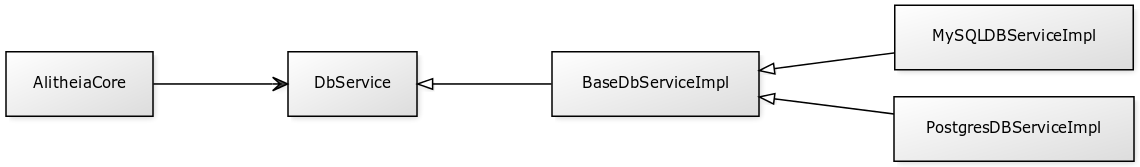
\includegraphics[width=0.8\textwidth]{dbs}
    \caption{Refactoring of DbServiceImpl. Only Postgres and MySQL driver are shown for brevity.}
    \label{fig:dbs}
\end{figure}

We compared the \verb|DbServiceImpl| and \verb|BaseDbServiceImpl| in the old and new architecture. Unfortunately, the only difference that inFusion recognized was the reduced number of public fields (from `many' to `none'). Though this was not our intention, it does indicate better use of encapsulation.

% TODO: Vertel over tabel hieronder

\begin{table}
	\centering
    \begin{tabular}{l|llll}
    ~                                 & Before & After & ~ & ~ \\ \hline
    Average operation complexity      & 2.51 & 2.51 \\
    Weighted method complexity        & 98   & 38 \\
    Number of cyclic dependencies     & 104  & 108 \\
    Number of dependencies            & 15   & 15  \\
    Number of dependants              & 1    & 6   \\
    \end{tabular}
    \caption{Metrics for AlitheiaCore}
\end{table}

\subsubsection{SRP: Providing a database}
We felt like it would be a good idea to extract the creating of the database out of \verb|AlitheiaCore| and into a \verb|DbServiceFactory|. This new class is responsible for creating the database depending on the system parameters. By extracting this code into a separate class we break up both dependencies and responsibilities. \verb|AlitheiaCore| is made to depend on this new class for the creating of a database.

\begin{figure}[h]
    \centering
    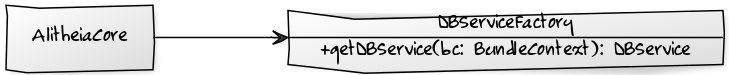
\includegraphics[width=0.8\textwidth]{dbfactory}
    \caption{Extracting DbService creation out of AlitheiaCore.}
    \label{fig:dbfactory}
\end{figure}

We ran Metrics Reloaded before and after applying these refactorings. We looked at the number of cyclic dependencies, number of dependencies, number of transitive dependencies and number of dependants. According to these results, the new class is less maintainble than the old class. However, we believe that this is a necessary consequence of separating responsibilities and breaking dependencies.

\begin{table}
	\centering
    \begin{tabular}{l|llll}
    ~                                 & Before & After & ~ & ~ \\ \hline
    Average operation complexity      & 1.36   & 1.35 \\
    Weighted method complexity        & 30     & 31 \\
    Number of cyclic dependencies     & 104 & 108 \\
    Number of dependencies            & 25  & 26  \\
    Number of dependants              & 55  & 59  \\
    \end{tabular}
    \caption{Metrics for AlitheiaCore}
\end{table}

\subsection{Test coverage}
While refactoring our code we wrote tests to ensure that we would not break the functionality. Our tests make extensive use of Mockito\footnote{\url{https://github.com/mockito/mockito}} to mock dependencies. To assess the effectiveness of our test harness, we investigated the test coverage before and after our refactorings. Table~\ref{tbl:coverage} reports the test coverage for packages that are relevant to our changes.

\begin{table}[h]
	\centering
    \begin{tabular}{ll|lll}
    ~                           & ~      & Class      & Method       & Line         \\ \hline
    eu.sqooss.impl.service.db   & Before & 0\% (0/2)  & 0\% (0/41)   & 0\% (0/417) \\
    ~                           & After  & 85\% (6/7) & 12\% (8/62)  & 5\% (25/433) \\ \hline
    eu.sqooss.service.db        & Before & 0\% (0/52) & 0\% (0/697)  & 0\% (0/2107) \\
    ~                           & After  & 9\% (5/53) & 1\% (10/698) & 1\% (38/2108) \\ \hline
    eu.sqooos.service.scheduler & Before & 75\% (3/4) & 29\% (17/57) & 21\% (62/291) \\
    ~                           & After  & 80\% (4/5) & 32\% (19/59) & 28\% (83/294) \\ \hline
    eu.sqooos.service.cache     & Before & 50\% (2/4) & 31\% (7/22)  & 33\% (48/145) \\
    ~                           & After  & 75\% (3/4) & 36\% (8/22)  & 38\% (51/133)

    \end{tabular}
    \caption{Test coverage for relevant packages}
    \label{tbl:coverage}
\end{table}

\bibliographystyle{plain}
\bibliography{report}

\end{document}